\documentclass[a4paper]{article}
\usepackage[
	pdftex,
	colorlinks=true,
	bookmarksnumbered=true,
	bookmarksopen=true,
	bookmarksopenlevel=3,
	pdfstartview=FitP,
	urlcolor=blue,
]{hyperref}
\pdfinfo{
	/Title(Esercitazione di Laboratorio: Arduino)
	/Author(Coa Giulio, Licastro Dario, Montano Alessandra)
}
\usepackage[italian]{babel}
\usepackage{amsmath,geometry,graphicx,listings,mdsymbol,stmaryrd,subcaption,titling,xcolor}
\definecolor{comment}{rgb}{1, 0.83, 0}
\lstset{
	backgroundcolor = \color{white},
	basicstyle = \ttfamily \footnotesize \color{black},
	breakatwhitespace = false,
	breaklines = true,
	captionpos = b,
	columns = flexible,
	commentstyle = \color{comment},
	escapeinside = {\%*}{*)},
	frame = tb,
	keepspaces = true,
	keywordstyle = \color{blue},
	language = C++,
	numbers = left,
	numbersep = 5pt,
	numberstyle = \tiny\color{black},
	showspaces = false,
	showstringspaces = false,
	showtabs = false,
	stepnumber = 1,
	stringstyle = \color{red},
	tabsize = 1
}
\graphicspath{{./Image/}}
\renewcommand\maketitlehooka{
	\null
	\mbox{}
	\vfill
}
\renewcommand\maketitlehookd{
	\vfill
	\null
}
\title{
	\begin{center}
		Esercitazione di Laboratorio:
	\end{center}
	\newline
	\begin{center}
		Arduino
	\end{center}
}
\author{
	Coa Giulio (s236723)
	\and
	Licastro Dario (s234421)
	\and
	Montano Alessandra (s238160)
}
\begin{document}
	%-----------------------------------------------------------------------------
	%  TITLE
	%-----------------------------------------------------------------------------
	\begin{titlingpage}
		\maketitle
	\end{titlingpage}
	\newpage
	%-----------------------------------------------------------------------------
	%  PURPOSE OF THE EXPERIENCE
	%-----------------------------------------------------------------------------
	\section{Scopo dell'esperienza}
		Lo scopo di questa esercitazione è sviluppare un termometro digitale tramite l'uso di un sensore di temperatura e di una scheda Arduino.
	%-----------------------------------------------------------------------------
	%  INSTRUMENTATION USED
	%-----------------------------------------------------------------------------
	\section{Strumentazione utilizzata}
		La strumentazione usata durante l'esercitazione è:
		\begin{center}
			\begin{tabular}{ |c|c|c| }
				\hline
				\multirow{\textbf{Strumento}}	 		   & \textbf{Marca e Modello} & \textbf{Caratteristiche} \\
				\hline
				\multirow{Multimetro}			 		   & Agilent 34401A			  & \\
				\multirow{Oscilloscopio}		 		   & Rigol DS1054Z			  & 4 canali, \\
												 		   &						  & $ B = 50 \, \mathrm{MHz} $, \\
												 		   &						  & $ f_{\mathrm{c}} = 1 \, \mathrm{G\frac{Sa}{s}} $, \\
												 		   &						  & $ R_{\mathrm{i}} = 1 \, \mathrm{M\Omega} $, \\
												 		   &						  & $ C_{\mathrm{i}} = 13 \, \mathrm{pF} $, \\
												 		   &						  & $ 12 \, \mathrm{Mbps} $ di profondità di memoria \\
				\multirow{Generatore di segnali} 		   & Rigol DG1022			  & 2 canali, \\
												 		   &						  & $ f_{\mathrm{uscita}} = 20 \, \mathrm{MHz} $, \\
												 		   &						  & $ Z_{\mathrm{uscita}} = 50 \, \mathrm{\Omega} $ \\
				\multirow{Scheda Arduino}	 		   	   & UNO					  & $ f_{\mathrm{c, max}} = 76.9 \, \mathrm{k\frac{Sa}{s}} $ \\
				\multirow{Sensore di temperatura}	 	   & LM335					  & $ S = 10 \, \mathrm{m\frac{V}{K}} $, \\
														   &						  & $ V_{\mathrm{out}} = 0 \, \mathrm{V} $ @ $ 0 \, \mathrm{K} $ \\
														   &						  & $ \delta T = \pm 2 \, \mathrm{\text{\textdegree}C} $ \\
														   &						  & Campo di temperatura pari a $ -40 \div 100 \, \mathrm{\text{\textdegree}C} $ \\
														   &						  & Resistenza termica pari a $ 165 \, \mathrm{\frac{\text{\textdegree} C}{W}} $ \\
				\multirow{Cavi coassiali}		 		   &						  & Capacità dell'ordine dei $ 80 \div 100 \, \mathrm{p\frac{F}{m}} $ \\
				\multirow{Connettori}			 		   &						  & \\
				\hline
			\end{tabular}
		\end{center}
	%-----------------------------------------------------------------------------
	%  THEORETICAL PREMISES
	%-----------------------------------------------------------------------------
	\section{Premesse teoriche}
		\subsection{Incertezza sulla misura dell'oscilloscopio}
			La misura del valore di un segnale tramite l’oscilloscopio (sia esso l'ampiezza, la frequenza, il periodo, etc.) presenta un'incertezza che dipende, principalmente, da due fattori:
			\begin{itemize}
				\item l’incertezza strumentale introdotta dall’oscilloscopio (ricavabile dal manuale).
				\item l’incertezza di lettura dovuta all’errore del posizionamento dei cursori.
			\end{itemize}
			Quest’ultima incertezza deriva dal fatto che il segnale visualizzato non ha uno spessore nullo sullo schermo.
		\subsection{Arduino}
			Arduino è una piattaforma elettronica open surce basata su un hardware di facile utilizzo e programmabie in un ambiente software dedicato.
			\subsubsection{Arduino UNO}
				Arduino UNO è una scheda composta da un convertitore ADC a $ 10 $ bit ($ 8 $ bit se la frequenza d'utilizzo è maggiore di $ 15 \, \mathrm{k\frac{Sa}{s}} $) che può essere alimentato da due distinte sorgenti, una interna alla scheda da $ 1.1 \pm 0.1 \, \mathrm{V} $ e una esterna da $ 5 \pm 0.25 \, \mathrm{V} $ ($ 4.85 \pm 0.4 \, \mathrm{V} $ se si usa la porta USB 3.0 anzichè la porta USB 2.0).
				\begin{figure}[h!]
					\centering
					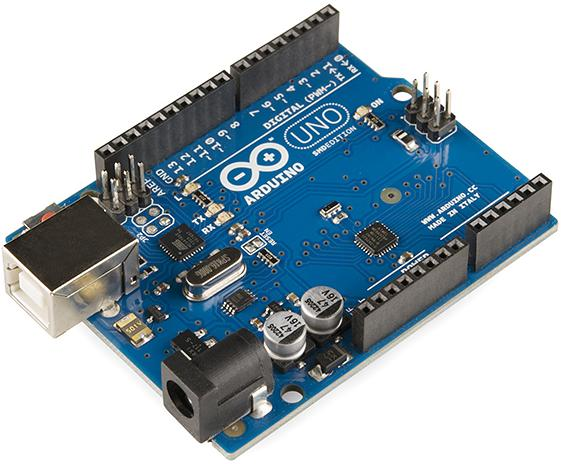
\includegraphics[scale=0.6]{ArduinoUNO}
					\caption{Arduino UNO.}
					\label{fig:ArduinoUNO}
				\end{figure}
		\subsection{Sensore LM335}
			Il sensore LM335 è un sensore di temperatura prodotto dalla National Semiconductor; esso permette di avere in uscita una tensione proporzionale alla temperatura rilevata ($ V_{\mathrm{out}} = S \cdot T_{\mathrm{K}} $).
			\newline
			Il suo comportamento è assimilabile a quello di un diodo di Zener la cui corrente $ I_{\mathrm{D}} $ deve essere compresa nell'intervallo $ 0.4 \, \mathrm{mA} \div 5 \, \mathrm{mA} $.
			\begin{figure}[h!]
				\centering
				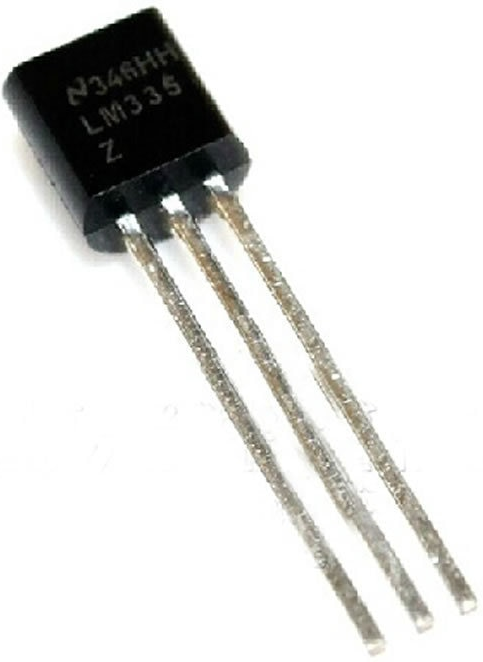
\includegraphics[scale=0.2]{LM335}
				\caption{Sensore LM335.}
				\label{fig:LM335}
			\end{figure}
		\subsection{Other}
			.
	%-----------------------------------------------------------------------------
	%  LABORATORY EXPERIENCE
	%-----------------------------------------------------------------------------
	\section{Esperienza in laboratorio}
		\subsection{Circuito di condizionamento}
			Per i nostri scopi, il sensore LM335 deve lavorare lavorare in regione di polarizzazione inversa, percui esso verrà utilizzato con il catodo collegato alla massa e con l'anodo collegato alla sorgente di tensione.
			\newline
			Al fine di garantire un corretto funzionamento del sensore, dobbiamo garantire che la corrente che vi circola all'interno sia nel range di funzionamento; a tale scopo applichiamo una resistenza $ R_{1} $ a monte del diodo, di modo che la corrente che scorra nel diodo rientri nel suddetto range.
			\begin{figure}[h!]
				\centering
				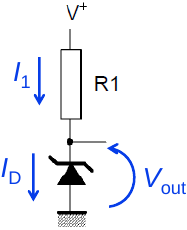
\includegraphics[scale=0.5]{circuitoDiCondizionamento}
				\caption{Circuito di condizionamento.}
				\label{fig:circuitoDiCondizionamento}
			\end{figure}
		\subsection{Misura della temperatura}
			\begin{lstlisting}
				#include <string.h>
				
				//#define INT
				
				int pin, time, D_out, N_B;
				float S, T_C, T_K, V_out, V_FR;
				
				void setup() {
					Serial.begin(9600);	// setup Serial
					pin = A0;	// set the pin to read data
					time = 1000;	// set how much time the sensor must execute the measurement of the temperature
					S = 10 * pow(10, -3);
					N_B = 10;
					V_FR = 4.9;
					#ifdef INT
						analogReference(INTERNAL);	// set the type of alimentation
					#endif
				}
				void loop(){
					D_out = analogRead(pin);	// read data from the pin
					T_K = D_out * V_FR / pow(2, N_B) * 1 / S;
					T_C = T_K - 273.15;
					V_out = D_out * V_FR / pow(2, N_B);
					Serial.println("D_out: " + String(D_out) + " -- V_out: " + String(V_out) + " V -- T: " + String(T_K) + " K -- T: " + String(T_C) + " %*\color{red} \textdegree*)C");
					delay(time);
				}
			\end{lstlisting}
		\subsection{Stima dell'incertezza}
			.
		\subsection{Modifica del circuito di condizionamento}
			.
		\subsection{Firmware del micro-controllore}
			.
		\subsection{Caratterizzazione del sistema}
			.
	%-----------------------------------------------------------------------------
	%  RESULTS
	%-----------------------------------------------------------------------------
	\section{Risultati}
		\subsection{Circuito di condizionamento}
			In base ai dati fornitici, abbiamo proceduto al calcolo della tensione massima e della tensione minima a cui il sensore LM335 deve lavorare.
			\newline
			\begin{equation*}
				\begin{split}
					V_{\mathrm{out, max}} &= S \cdot T_{\mathrm{K, max}} = \\
										  &= S \cdot (T_{\mathrm{max}} + 273.15) = \\
										  &= 10m \cdot (50 + 273.15) = \\
										  &= 3.23 \, \mathrm{V}
				\end{split}
			\end{equation*}
			\begin{equation*}
				\begin{split}
					V_{\mathrm{out, min}} &= S \cdot T_{\mathrm{K, min}} = \\
										  &= S \cdot (T_{\mathrm{min}} + 273.15) = \\
										  &= 10m \cdot (5 + 273.15) = \\
										  &= 2.78 \, \mathrm{V}
				\end{split}
			\end{equation*}
			Essendo che la resistenza $ R_{1} $ è posta in serie al sensore, la corrente che scorre nel diodo è uguale a quella che scorre nella resistenza (in realtà è approssimabile, dato che si va a misurare la tensione ai capi del diodo e si ha un minimo di "perdite").
			\newline
			\begin{center}
				$ I_{\mathrm{D}} \approx I_{1} = \frac{V_{\mathrm{s}} - V_{\mathrm{out}}}{R_{1}} $
			\end{center}
			\newline
			Da ciò, si ha che le limitazioni sulla corrente che attraversa il diodo diventano
			\newline
			\begin{center}
				$ \frac{V_{\mathrm{s}} - V_{\mathrm{out, min}}}{R_{1}} > 0.4 \, \mathrm{mA} $
			\end{center}
			\newline
			\begin{center}
				$ \frac{V_{\mathrm{s}} - V_{\mathrm{out, min}}}{R_{1}} < 5 \, \mathrm{mA} $
			\end{center}
			\newline
			Da cui si ha che
			\newline
			\begin{center}
				$ \frac{V_{\mathrm{s}} - V_{\mathrm{out, min}}}{0.4m} > R_{1} > \frac{V_{\mathrm{s}} - V_{\mathrm{out, min}}}{5m} $
			\end{center}
			\newline
			\begin{center}
				$ 4425 \, \mathrm{\Omega} > R_{1} > 444 \, \mathrm{\Omega} $
			\end{center}
			Successivamente, abbiamo stimato la temperatura dell'ambiente in cui il diodo avrebbe lavorato, tenendo conto dell'autoriscaldamento del sensore, e, di conseguenza, la tensione in uscita che esso avrebbe prodotto.
			\begin{equation*}
				\begin{split}
					V_{\mathrm{out}} &= S \cdot T_{\mathrm{K}} = \\
									 &= S \cdot (T + 273.15) = \\
									 &= 10m \cdot (25 + 273.15) = \\
									 &= 2.98 = \\
									 &\approx 3 \, \mathrm{V}
				\end{split}
			\end{equation*}
			Ed abbiamo imposto che $ I_{\mathrm{D}} $ fosse di $ 2 \, \mathrm{mA} $, da cui
			\begin{equation*}
				\begin{split}
					R_{1} &= \frac{V_{\mathrm{s}} - V_{\mathrm{out}}}{I_{1}} = \\
						  &= \frac{5 - 3}{2m} = \\
						  &= 1 \, \mathrm{k\Omega}
				\end{split}
			\end{equation*}
		\subsection{Misura della temperatura}
			\begin{lstlisting}
				#include <string.h>
				
				//#define INT
				
				int pin, time, D_out, N_B;
				float S, T_C, T_K, V_out, V_FR;
				
				void setup() {
				Serial.begin(9600);	// setup Serial
				pin = A0;	// set the pin to read data
				time = 1000;	// set how much time the sensor must execute the measurement of the temperature
				S = 10 * pow(10, -3);
				N_B = 10;
				V_FR = 4.9;
				#ifdef INT
				analogReference(INTERNAL);	// set the type of alimentation
				#endif
				}
				void loop(){
				D_out = analogRead(pin);	// read data from the pin
				T_K = D_out * V_FR / pow(2, N_B) * 1 / S;
				T_C = T_K - 273.15;
				V_out = D_out * V_FR / pow(2, N_B);
				Serial.println("D_out: " + String(D_out) + " -- V_out: " + String(V_out) + " V -- T: " + String(T_K) + " K -- T: " + String(T_C) + " %*\color{red} \textdegree*)C");
				delay(time);
				}
			\end{lstlisting}
		\subsection{Stima dell'incertezza}
			.
		\subsection{Modifica del circuito di condizionamento}
			.
		\subsection{Firmware del micro-controllore}
			.
		\subsection{Caratterizzazione del sistema}
			.
\end{document}